%%========================================================================
%% LaTeX sjabloon voor stage/projectrapport of bachelorproef
%%  HoGent Bedrijf en Organisatie
%%========================================================================

%%========================================================================
%% Preamble
%%========================================================================

\documentclass[pdftex,a4paper,12pt,twoside]{report}

% XXX: Let op: dit sjabloon is gemaakt om dubbelzijdig af te drukken
% Voor enkelzijdig, verwijder ``twoside'' hierboven.

%%---------- Extra functionaliteit ---------------------------------------

\usepackage[utf8]{inputenc}  % Accenten gebruiken in tekst (vb. é ipv \'e)
\usepackage{amsfonts}        % AMS math packages: extra wiskundige
\usepackage{amsmath}         %   symbolen (o.a. getallen-
\usepackage{amssymb}         %   verzamelingen N, R, Z, Q, etc.)
\usepackage[dutch]{babel}    % Taalinstellingen: woordsplitsingen,
                             %  commando's voor speciale karakters
                             %  ("dutch" voor NL)
\usepackage{eurosym}         % Euro-symbool €
\usepackage{geometry}
\usepackage{graphicx}        % Invoegen van tekeningen
\usepackage[pdftex,bookmarks=true]{hyperref}
                             % PDF krijgt klikbare links & verwijzingen,
                             %  inhoudstafel
\usepackage{listings}        % Broncode mooi opmaken
\usepackage{multirow}        % Tekst over verschillende cellen in tabellen
\usepackage{rotating}        % Tabellen en figuren roteren
\usepackage{natbib}          % Betere bibliografiestijlen
\usepackage{fancyhdr}        % Pagina-opmaak met hoofd- en voettekst

\usepackage[T1]{fontenc}     % Ivm lettertypes
\usepackage{lmodern}
\usepackage{textcomp}

\usepackage{lipsum}          % Voor vultekst (lorem ipsum)

\usepackage{wrapfig}

%%---------- Layout ------------------------------------------------------

% hoofdingen, enz.
\pagestyle{fancy}
% enkel hoofdstuktitel in hoofding, geen sectietitel (vermijd overlap)
\renewcommand{\sectionmark}[1]{}

% lijn, wordt gebruikt in titelpagina
\newcommand{\HRule}{\rule{\linewidth}{0.5mm}}

% Leeg blad
\newcommand{\emptypage}{
\newpage
\thispagestyle{empty}
\mbox{}
\newpage
}

% Gebruik een schreefloos lettertype ipv het "oubollig" uitziende
% Computer Modern
\renewcommand{\familydefault}{\sfdefault}

% Commando voor invoegen Java-broncodebestanden (dank aan Niels Corneille)
% Gebruik: \codefragment{source/MijnKlasse.java}{Uitleg bij de code}
\newcommand{\codefragment}[2]{ \lstset{%
  language=java,
  breaklines=true,
  float=th,
  caption={#2},
  basicstyle=\scriptsize,
  frame=single,
  extendedchars=\true
}
\lstinputlisting{#1}}

%%---------- Documenteigenschappen ---------------------------------------
%% Vul dit aan met je eigen info:

% Je eigen naam
\newcommand{\student}{Ritchie Van Mele}

% De naam van je lector, begeleider, promotor
\newcommand{\promotor}{Johan Decorte}

% De naam van je co-promotor
\newcommand{\copromotor}{Krist Vanneste}

% Indien je bachelorproef in opdracht van een bedrijf of organisatie
% geschreven is, geef je hier de naam.
\newcommand{\instelling}{Hogeschool Gent}

% De titel van het rapport/bachelorproef
\newcommand{\titel}{Wat is VOIP, hoe beveilig ik mijn netwerk hiervoor en hoe werkt het met IPV6}

% Datum van indienen
\newcommand{\datum}{29 mei 2015}

% Faculteit
\newcommand{\faculteit}{Faculteit Bedrijf en Organisatie}

% Soort rapport
\newcommand{\rapporttype}{Scriptie voorgedragen tot het bekomen van de graad van\\Bachelor in de toegepaste informatica}

% Academiejaar
\newcommand{\academiejaar}{2014-2015}

% Examenperiode
%  - 1e semester = 1e examenperiode
%  - 2e semester = 2e examenperiode
%  - tweede zit = 3e examenperiode
\newcommand{\examenperiode}{Tweede examenperiode}

%%========================================================================
%% Inhoud document
%%========================================================================

\begin{document}

%%---------- Front matter ------------------------------------------------
%% Het voorblad - Hier moet je in principe niets wijzigen.

\begin{titlepage}
  \newgeometry{top=2cm,bottom=1.5cm,left=1.5cm,right=1.5cm}
  \begin{center}

    \begingroup
    \rmfamily
    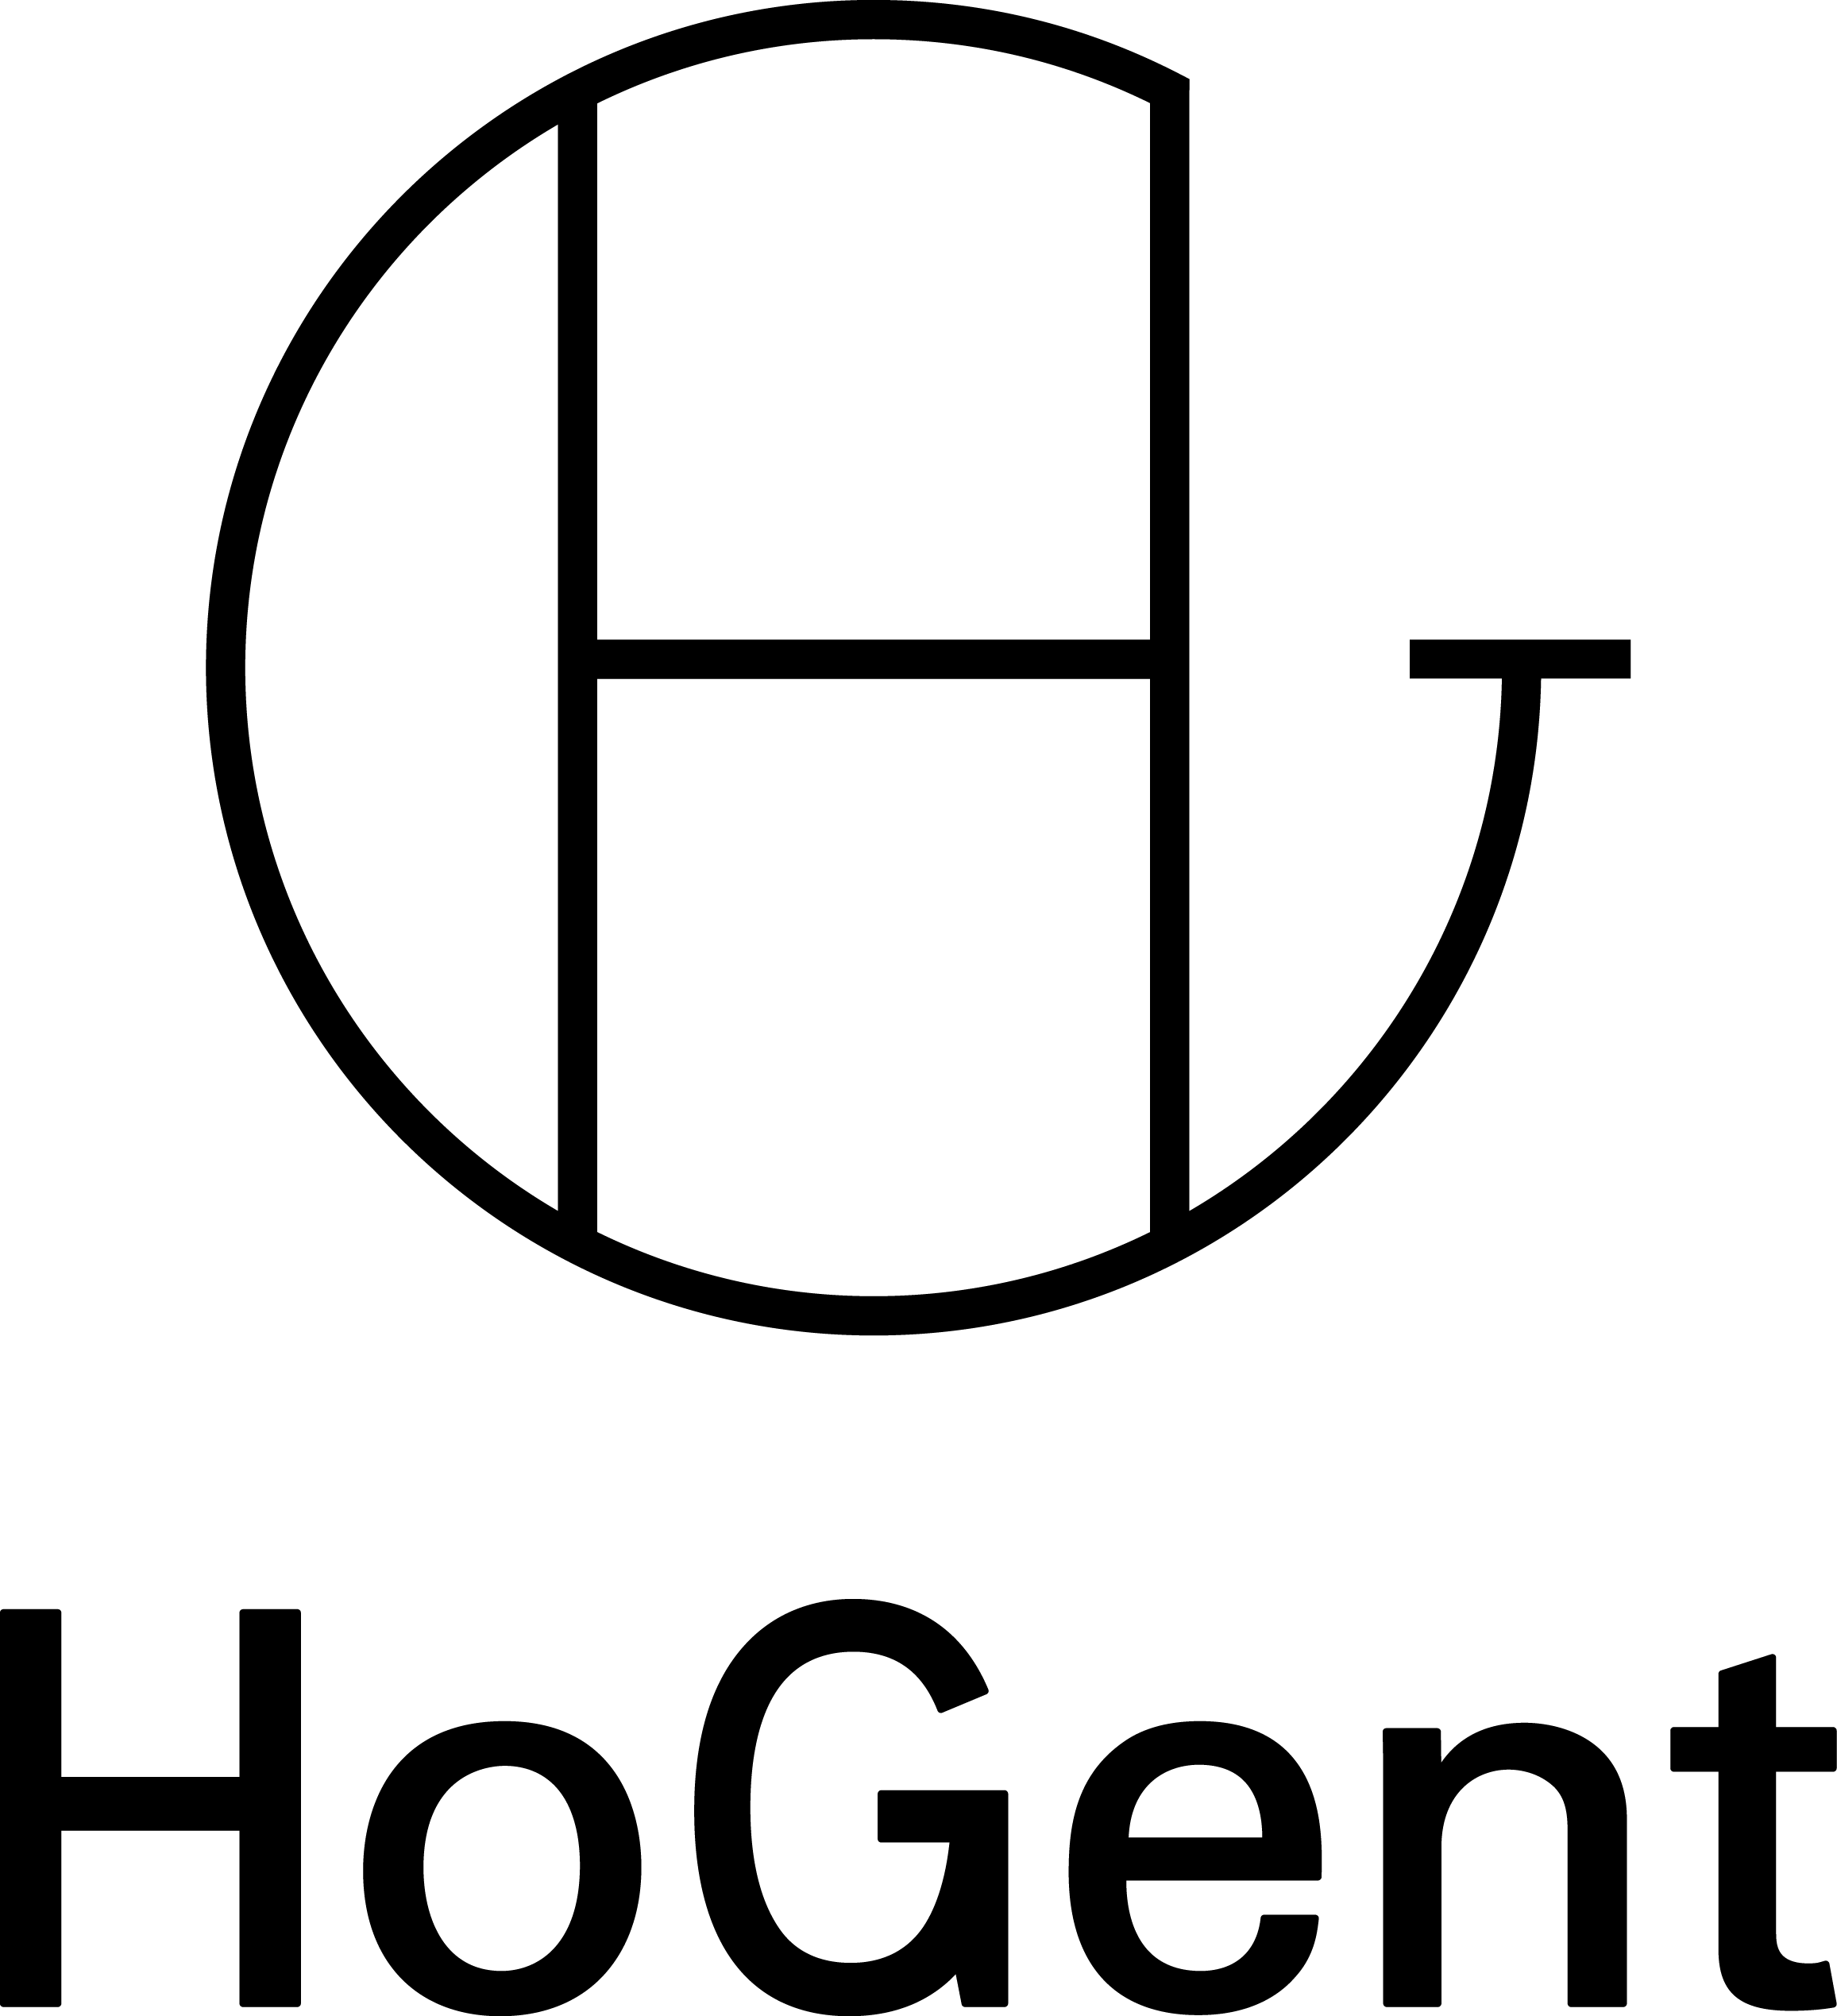
\includegraphics[width=2.5cm]{img/HG-beeldmerk-woordmerk}\\[.5cm]
    \faculteit\\[3cm]
    \titel
    \vfill
    \student\\[3.5cm]
    \rapporttype\\[2cm]
    Promotor:\\
    \promotor\\
    Co-promotor:\\
    \copromotor\\[2.5cm]
    Instelling: \instelling\\[.5cm]
    Academiejaar: \academiejaar\\[.5cm]
    \examenperiode
    \endgroup

  \end{center}
  \restoregeometry
\end{titlepage}

% Schutblad

\emptypage


\begin{titlepage}
  \newgeometry{top=5.35cm,bottom=1.5cm,left=1.5cm,right=1.5cm}
  \begin{center}

    \begingroup
    \rmfamily
    \faculteit\\[3cm]
    \titel
    \vfill
    \student\\[3.5cm]
    \rapporttype\\[2cm]
    Promotor:\\
    \promotor\\
    Co-promotor:\\
    \copromotor\\[2.5cm]
    Instelling: \instelling\\[.5cm]
    Academiejaar: \academiejaar\\[.5cm]
    \examenperiode
    \endgroup

  \end{center}
  \restoregeometry
\end{titlepage}


\begin{abstract}
% TODO: De "abstract" of samenvatting is een kernachtige (max 1 blz. voor een
% thesis) synthese van het document. In ons geval beschrijf je kort de
% probleemstelling en de context, de onderzoeksvragen, de aanpak en de
% resultaten.

Deze bachlorproef draait rond voice over IP(VOIP). In deze proef stel ik mezelf vragen en tracht daarop antwoorden te vinden. Ik ga trachten duidelijk te maken wat VOIP is en hoe ze verschilt van traditionele telefonie. Bij VOIP wordt de telefonie over een netwerk gestuurd. Ik ga dan ook onderzoeken welke invloed VOIP heeft op dit netwerk en of dit een probleem geeft voor je beveiliging. Beveiliging zowel t.o.v. het bestaande netwerk maar ook ten opzichte van je telefonie. Dan ga ik ook kijken naar op welke manieren je een onbeveiligd VOIP netwerk kan misbruiken en hoe je te beschermen tegen deze praktijken. De bedoeling is dat je na het lezen van deze proef weet wat VOIP is met alle voor en nadelen. Hoe het veilig en onveilig is en hoe je te beschermen tegen inbreuken. Deze proef sluit aan bij mijn stage bij SmartTelecom NV. Hier implementeer en beheer VOIP in nieuwe en bestaande netwerken bij klanten. Op deze manier kom ik dagelijks in contact met de voor en nadelen van VOIP. Alsook met de gevaren ervan en hoe te beveiligen tegen deze gevaren. Research via deze stage is dan ook mijn voornaamste aanpak van de probleemstelling.
 
\end{abstract}

\chapter*{Voorwoord}
\label{ch:voorwoord}
Deze thesis is in het kader van mijn bachlorproef voor toegepaste informatica aan de hogeschool Gent.\\
Ik wil mijn stagementor en copromotor Krist Vanneste van SmartTelecom NV bedanken voor de hulp en research mogelijk door hem.\\
Ook bedank ik mijn stage partner Dries Vandooren voor de nuttige invloed tijdens de stage en in het onderwerp VOIP.
% TODO: Vergeet ook niet te bedankten wie je geholpen/gesteund/... heeft

\tableofcontents

% Als je een lijst van afkortingen of termen wil toevoegen, dan hoort die
% hier thuis. Gebruik bijvoorbeeld de ``glossaries'' package.

%%---------- Kern --------------------------------------------------------

\chapter{Inleiding}
\label{ch:inleiding}

Wat is VOIP? VOIP of Voice Over IP(Internet Protocol) is de technologie waar je telefonie en multimedia sessies(conference call met beeld) gaat sturen over een IP netwerk. Men verwijst vaak naar VOIP als internet telefonie. Hierbij ga je je communicatie(stem, sms, fax, … ) sturen over het internet in tegenstelling tot bij traditionele telefonie waarbij dit via een public telefonie netwerk gebeurde. In tegenstelling tot wat de naam zegt is internet verbinding niet altijd nodig bij VOIP. VOIP betekend eenvoudig dat je je communicatie gaat versturen via dezelfde protocollen als degene het internet gebruikt. Zo kan je binnen een groot bedrijf elke werknemer voorzien van VOIP telefoons en deze kunnen elkaar bellen via VOIP zonder dat ze verbinding maken met het internet. Eens ze willen bellen naar locaties buiten hun netwerk dan komt er uiteraard internet aan te pas.\\ \\
Maar we lopen vooruit op de feiten. We starten met telefonie waar het allemaal bij startte. De eerste telefoons. De eerste telefoonlijn was een directe lijn tussen 2 toestellen. Eens er meer en meer toestellen kwamen maakte men gebruik van POTS wat staat voor “Plain Old Telephone Service”. Vertaalt is dit “de eenvoudig oude telefoon service”. POTS ging over een netwerk genaamd PSTN(“public switched telephone network” of ” publiek verdeeld telefoon netwerk”). Bij directe verbindingen tussen toestellen was er sprake van een analoog signaal tussen de 2. De stem werd op deze manier overgebracht. POTS en PSTN werden mogelijk toen de ontdekking werd gemaakt dat men dit analoog signaal kon omvormen naar een digitaal signaal. Een stem die in origine analoog was kon worden omgevormd naar een digitaal signaal en kon worden verstuurd als nullen en eentjes. Een betere technologie was ontwikkeld en de basis voor wat later zou uitgroeien tot VOIP was gelegd. \\ \\
Tot op dat moment werd er gekozen om de telefonie gescheiden te houden van het opkomende computernetwerk. In computernetwerken werd er gewerkt met pakketten. Om VOIP gebruik te laten maken van deze netwerkten zou het ook zo gaan werken. VOIP gaat de geluidssignalen opsplitsen in pakketten en deze versturen over het netwerk. Deze pakketten bevatten behalve het geluid signaal ook het netwerk adres van de beller en ontvanger. En door het gebruik van pakketten werd het mogelijk om meer informatie mee te sturen om de communicatie te ondersteunen en verbeteren. \\ \\
Waar POTS specifieke benodigdheden had is VOIP enorm veelzijdig. Het werkt op verscheidene soorten netwerken. En het werkt niet alleen met VOIP telefoons maar ook met computers, Pda’s en zelf smartphones. Deze toestellen bevatten allemaal een NIC( Network Interface Card) net zoals een computer. Via deze NIC’s krijgen de toestellen dan een netwerk adres(IP-adres). Op deze manier zijn VOIP toestellen deel van je computer netwerk. \\ \\
Wat zijn nu de voor en nadelen van POTS en VOIP.\\

POTS: 
\begin{itemize}
	\item voordelen
	\begin{itemize}
		\item Het is in vele gevallen al aanwezig.
	\end{itemize}
	\item nadelen
	\begin{itemize}
		\item Het aantal main telefoonlijnen is het aantal oproepen je bedrijf tegelijk aankan. 
		\item Het aantal extenties je kan hebben is bepaald door je PBX( private branch exchange)
		\item Het werkt enkel met analoge telefoons. Geen pc's, smartphones, \ldots
	\end{itemize}
\end{itemize} 
VOIP: 
\begin{itemize}
	\item voordelen
	\begin{itemize}
		\item Ongelimiteerd aantal oproepen dat je tegelijk kan afhandelen(als je internet snel genoeg is)
		\item Ongelimiteerd aantal extenties.
		\item Bied meer aan dan enkel telefonie zoals Video calls,bellen vanop PC's, \ldots
		\item Geen gescheiden netwerk voor telefonie(geen dubbele bekabeling)
	\end{itemize}
	\item nadelen
	\begin{itemize}
		\item Er is een investeringskost bij aankoop van toestellen en PBX
	\end{itemize}
\end{itemize} 

Het is dus zeer duidelijk dat de overstap maken naar VOIP een zeer goede stap is voor bedrijven. Het geeft hen meer opties en de voordelen wegen meer door dan de nadelen. \\
Eens een bedrijf de stap maakt naar een Voice over Internet Protocol systeem is er nog een beslissing die te nemen is. Kies je voor een hosted Voip of voor een niet hosted voip.
In de voorgaande analyse ging ik er van uit dat alle apparatuur zich on site bevond. Dit wil zeggen dat alle apparatuur zoals telefoons en PBX zich op de locatie van het bedrijf bevinden.
Dit is niet de eenige mogelijkheid. Je kan er ook voor kiezen om je PBX te laten hosten door een hosting bedrijf. Hierbij zullen je VOIP telefoons geen verbinding maken met een PBX binnen je netwerk.
Maar met een PBX centrale die zich op het internet bij een bedrijf die de diensten van hun PBX aanbied. Op deze manier kan je als bedrijf kosten sparen door de aankoop van een eigen PBX systeem te vervangen door een maandelijkse hosting kost.
De voordelen van een hosted VOIP zijn dat je geen grote aankoopkost hebt, alsook dat je geen onderhoudskosten hebt. Ook kan je hierbij je VOIP telefoon toestellen plaatsen waar je wil. Je kan je toestel na het werk meenemen naar huis en daar berijkbaar zijn op het nummer van op werk.
Bij een beheren van je eigen PBX is er een investering in materiaal, maar dit geeft je de mogelijkheid je VOIP netwerk te beheren zoals jij dat wil. In theorie zou je verbindingen kunnen open stellen waarbij je je toestel ook zou kunnen thuis zetten. Dit wordt wel afgeraden omdat dit je netwerk midner veilig maakt. Meer informatie later in deze thesis.
\\
Als we naar al deze voor en nadelen kijken en we zien alle extra's dat VOIP aanbied, dan is alles positief. Nu is de vraag of en hoe VOIP dit allemaal kan. Om te begrijpen hoe VOIP werkt gaan we kijken naar een model dat al lang word gebruikt op het internet namelijk het TCP/IP model. Het TCP/IP model is een aangepaste variant van het OSI model.
TCP/IP is een groep van netwerk protocollen. En een protocol is een regel die bepaald verkeer over een netwerk gaat regelen. Je hebt protocollen voor gewoon dataverkeer en je hebt er die strikt dienen voor VOIP. Elk van die protocollen komt overeen met een laag van het TCP/IP model. Ik ga de verschillende lagen niet beschrijven tenzij het nodig is om alles te begrijpen.
Een pakket zal van start tot einde van zijn tocht elke laag 2 maal doorlopen. Eenmaal bij het verzenden en eenmaal bij het ontvangen. Waar een normaal pakket vertrekt bij de verzendende pc en aankomt bij de ontvangende computer. Vertrekt een VOIP pakket bij de beller en komt aan bij de gebelde.
Het Pakket vertrekt bij de applicatielaag en elke laag dat het doorloopt krijgt het meer informatie en veranderd het van formaat. Eens het bij de onderste laag komt(Netwerk interface) dan wordt het verstuurd over het netwerk. Eens aangekomen bij de applicatielaag van de gebelde, wordt het omgezet naar een hoorbaar formaat.
\\
Natuurlijk zijn er verschillen tussen het normale dataverkeer en VOIP verkeer. In de bovenste laag(Applicatie laag) maakt VOIP gebruik van 3 protocollen:

\begin{itemize}
	\item NTP: Network Time protocol: Dit gaat de timing verzorgen bij het verzenden van de pakketen zodat alles gebeurd in de juiste volgorde en op die manier de kwaliteit te garanderen.
	\item RTP: Real-time Transport Protocol: Gaat end-to-end netwerk transport functionaliteiten toevoegen.
	\item RTCP: Real-time Transport Control Protocol: Dit gaat het geluids signaal controleren op aflevering en controle functies toevoegen.
\end{itemize}

Ook in de transport laag is er een verschil. Waar traditionele datapakketten gebruik maken van TCP, gaat VOIP net zoals Videoconferencing gebruik maken van UDP(user datagram protocol). TCP is een trager protocol dan UDP, dit is omdat TCP meer controleerd op ontvangst van pakketten. UDP is sneller omdat het dit niet doet. 
Als er bij normaal dataverkeer een aantal pakketten niet aankomt dan is er een probleem. Dan zijn er documenten of gegevens niet volledig. Bij VOIP mag er al eens een pakket wegvallen. Zelf al wou je het pakket opnieuw verzenden dan nog kan je dat niet. Gesproken taal is sequentieel en je kan dus een deel van het begin niet op het einde erbij plakken.
Daarom is er dus gekozen voor UDP. 



\begin{figure}[h]
\caption{Het OSI model naast het TCP/IP model.}
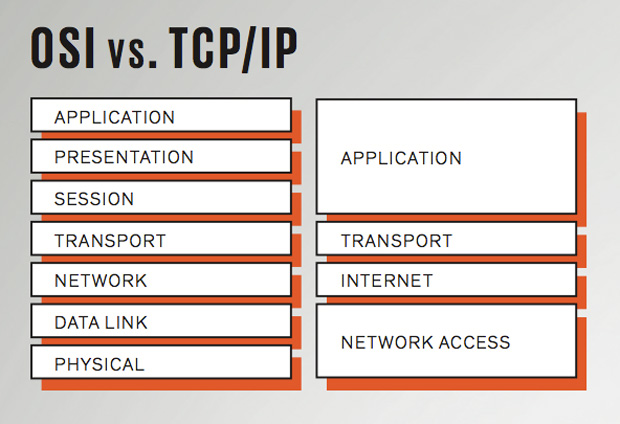
\includegraphics[scale=0.8]{img/TCP}
\end{figure}


\newpage

\section{Probleemstelling en Onderzoeksvragen}
\label{sec:onderzoeksvragen}
VOIP is een nieuwe technologie, en een nieuwe technologie toevoegen aan je netwerk levert mogelijk problemen op. 
Zoals eerder vermeld gebruikt VOIP het zelfde netwerk als je standaard netwerk data verkeer. Dit betekend dat alle beveiligingsrisico's en dreigingen dat gewoon verkeer heeft, dat deze ook dreigingen zijn voor VOIP. VOIP heeft, in tegendeel tot dataverkeer, nog geen echte standaard. Ook moet er bij VOIP rekening gehouden worden met QOS(quality of service). Een super veilig systeem met slechte kwaliteit van gesprekken is geen goed systeem. Er moet dus een middenweg gevonden worden om het systeem zo veilig mogelijk te maken zonder in te boeten aan QOS.
Nu ga ik dit alles opsplitsen in 3 categorieën.

\begin{itemize}
	\item Zijn er problemen in samenwerking met andere technologieën?
	\item Wat zijn de beveiligingsdreigingen van VOIP?
	\item Hoe werkt VOIP met IPV6?
\end{itemize}

\subsection{Samenwerking met andere Technologieën}

	\paragraph Kan VOIP ervoor zorgen dat de werking van je netwerk in het gedrang komt? Dan denk ik niet aan inbreuken via de VOIP maar eerder of de benodigdheden voor VOIP en de netwerklast die dit veroorzaakt problemen geeft voor de andere zaken die gebruik maken van het netwerk.

\subsection{Beveiligingsdreigingen}
Hier ga ik opsommen wat de voornaamste dreigingen zijn op het gebied van beveiliging van VOIP systemen.

	\paragraph Met behulp van packet sniffing software kan je de packetten van VOIP bekijken. Dit geeft je informatie over welk nummer op welk IP-address belt naar welk nummer. Deze informatie kan misbruikt worden. Door middel van bijvoorbeeld VOMIT,voice over misconfigured internet telephones, kan je de datastream van VOIP gesprekken omzetten naar een beluisterbaar formaat. 			Op deze manier kan je gesprek letterlijk worden afgeluisterd. Alle gevoelige informatie is dan dus niet meer veilig.

	\paragraph Zoals vroeger met traditionele telefonie is er bij VOIP ook altijd belang naar het verkrijgen van gratis telefonie. Men noemt dit phreaking. Hierbij gaat een fout individu trachten toegang te krijgen tot je VOIP netwerk. Op deze manier gaat deze persoon dan kunnen bellen op kosten van de eigenaar. Hij gaat dit trachten te doen door de authenticatiegegevens van een VOIP 			gebruikter te verkrijgen.

	\paragraph Indien je je netwerk veiliger maakte met de implementatie van een aparte vlan voor je VOIP telefonie is er de kans dat een individu gaat trachten toegang te krijgen tot je telefonie vlan door middel van VLAN hopping. 

	\paragraph Er zou iemand kunnen proberen om de gesprekken te verstoren. Dit is mogelijk door geluid pakketen te injecteren in de communicatie stream. Op deze manier kan de kwaliteit van een gesprek enorm verminderen, de twee sprekers kunnen zelf voor langere periodes stilte horen.

	\paragraph VOIP telefoons zijn zoals computers ook toestellen op je netwerk. Dit laat hen kwetsbaar voor een DOS aanval. Op deze manier kan iemand de telefoon spammen met onnodig veel SIP calls. Hierdoor wordt het toestel overbelast en kan het niet meer bellen of gebelt worden.

	\paragraph Waar traditionele telefoons een nummer hebben hebben VOIP telefoons een IP address. Traditionele telefoons krijgen soms reclame oproepen. Bij VOIP oproepen is het mogelijk om via scripts naar enorme hoeveelheden IP addressen reclame boodschappen te sturen. Degene toe terecht  komen bij toestellen zouden voor de zender voordelig zijn maar niet voor de eigenaar 			van dat toestel. Deze manier van reclame spamming noemt SPIT(Spamming over Internet Telephony).

 
\subsection{VOIP met IPV6}
	
	\paragraph Nu het duidelijk is dat we op het internet met een enorm tekort zitten aan publieke IP adressen is het dan ook geen verrassing dat er een nieuw internet protocol aankomt. Dit nieuwe protocol komt in de vorm van IPv6(Internet Protocol Versie 6). Elke overstap naar een nieuw protocol, van welke aard dan ook, brengt veranderingen met zich mee. Het zorgt voor vernieuwing 		maar het zorgt er ook voor dat je als gebruiker je netwerkinfrastructuur moet aanpassen zodat het met dit nieuwe protocol kan werken. \\
	Het is dan ook logisch dat we ons moeten afvragen wat de impact zal zijn van IPv6 op ons netwerk. En in het bijzonder de invloed op VOIP binnen ons netwerk? In dit deel zal ik onderzoeken wat de voordelen zijn voor VOIP en hoe we ons zullen moeten aanpassen om VOIP te laten werken met IPv6.

% TODO: Wees zo concreet mogelijk bij het formuleren van je
% onderzoeksvra(a)g(en). Een onderzoeksvraag is trouwens iets waar nog
% niemand op dit moment een antwoord heeft (voor zover je kan nagaan).

\chapter{Methodologie}
\label{ch:methodologie}


\paragraph Voor ik startte met mijn stage en mijn bachelor proef, was mijn kennis over VOIP vrij miniem. Ik wist in grote lijnen wat het deed maar niet zozeer hoe het dat deed. Mijn eerste stap naar het oplossen van mijn vragen was eenvoudig. Mijn stage is bij het bedrijf SmartTelecom NV. Dit bedrijf is een provider van VOIP systemen. Door mee te lopen met mijn stagementor Krist Vanneste kreeg ik als het ware een spoedcursus over VOIP. De eerste weken leerde ik hoe VOIP werkte en waar je op moest letten. Ik hielp met het implementeren van VOIP in zowel bestaande als nieuwe netwerken. Op deze manier kwam ik veel te weten over de praktijk van de zaak. Bijvoorbeeld dat bestaande netwerken soms niet optimaal zijn opgebouwd. Deze werken dan wel voor de basis toepassingen maar eens je er VOIP bij implementeerd zijn er problemen. 

\paragraph De tweede fase van mijn onderzoek was mijn bevindingen te gaan staven. Ik had ideeën over hoe VOIP in elkaar zit en waar je op moet letten bij het implementeren. Maar alvorens ik mijn bachelorproef kon beginnen schrijven moest ik uiteraard zorgen dat deze kennis correct was. Ik ben daarvoor aan het opzoeken geslaan. Ik ben beginnen opzoeken hoe VOIP werkt en wat experts zeggen dat de aandachtspunten zijn bij het opzetten van VOIP. Ik was dan ook zeer tevreden wanneer ik dit las en doorhad dat dit perfect aansloot met mijn eigen reeds vergaarde kennis.

\paragraph Waar ik bij het eerste en 2e deel de stage en opzoekwerk gesplitst deed deed ik bij mijn derde fase dit niet. In deze fase ging ik opzoek naar methoden om VOIP te misbruiken of om dit te dwarsbomen. Ik onderzocht hoe dit kon en hoe ik me ertegen kan beveiligen. Vervolgens ging ik dit controleren en implementeren bij een iets grotere klant. Deze klant is een bedrijvencentrum met vele verschillende partijen die toegang hebben tot het netwerk. Een zeer goede beveiliging was hier nodig en dit liet me toe om deze beveiligingen zelf te implementeren en te documenteren.



% TODO: Hoe ben je te werk gegaan? Verdeel je onderzoek in grote fasen, en
% licht in elke fase toe welke stappen je gevolgd hebt. Verantwoord waarom je
% op deze manier te werk gegaan bent. Je moet kunnen aantonen dat je de best
% mogelijke manier toegepast hebt om een antwoord te vinden op de
% onderzoeksvraag.


\chapter{Samenwerking met andere Technologieën}
\label{ch:Samenwerking met andere Technologieën}

\paragraph In theorie zorgt VOIP voor geen problemen met andere technologieën en zaken die van het netwerk gebruik maken. In de praktijk zie je dat niet elk netwerk geschikt is om VOIP te implementeren. \\
Zoals vele technologieën verlangt VOIP dat het netwerk sterk en krachtig genoeg is. Op een piekmoment van telefonie, kan VOIP veel vergen van de bandwith van je netwerk. Hier wordt het dus direct duidelijk dat zwakke en zeer eenvoudige netwerken problemen kunnen hebben met de benodigdheden van VOIP. \\
Als we een netwerk gaan analyseren kijken we naar het volgende.

\begin{itemize}
	\item Latency: Dit is de tijdsvertraging die optreed tussen de verzender en ontvanger. Bij VOIP mag dit maximum 150ms zijn. Meer zou ervoor zorgen dat het gesprek wegvalt. Latency kan worden veroorzaakt door elk netwerk apparaat waar pakketten door gestuurd worden. En als een apparaat druk belast wordt dan kan dit zorgen voor vertraging.
	\item Jitter: Jitter is de variatie in Latency die kan voorkomen in een netwerk. De latency is niet constant het zelfde. Jitter is dus een soort van standaard afwijking. Bij VOIP blijft de jitter best onder 50ms. Vanaf hogere waarden is er een grote impact op de QOS.
	\item Packetloss: Soms komen bepaalde pakketten niet aan op hun bestemming. Dan spreken we van Packet Loss. Voor VOIP kan je  maximum 1\% verlies toestaan bij WAN en slechts 0.05\% bij LAN. Packet loss zorgt ondermeer voor een hogere Jitter, wat dan weer voor slechte QOS zorgt. 
\end{itemize}
Als een van deze waarden hun grens overschrijdt dan zal de kwaliteit van het gesprek enorm achteruitgaan. Er moet dus gezorgd worden dat het netwerk snel genoeg is en dat het goed is opgebouwd. Zodat het VOIP aankan. \\
Vervolgens wordt duidelijk hoe VOIP andere technologieën kan tegenwerken. Als je in je netwerk gebruikmaakt van zaken die zelf ook veel bandwidth gebruiken. Dan kan een veeleisend VOIP met deze technologieën gaan vechten. Op deze manier leiden beide hieronder en gaan de werking van beiden achteruit. 


%% TODO: de structuur en titel van deze hoofdstukken hangen af van je
% eigen onderzoek. Elke fase in je onderzoek kan een eigen hoofdstuk krijgen. Kies telkens een gepaste titel. ``Corpus'' is *GEEN* gepaste titel

\chapter{Beveiligingsdreigingen}
\label{ch:Beveiligingsdreigingen}

\section{Packet Sniffing}

\paragraph In de wereld van netwerken bestaat er een term genaamd packet sniffing. Dit betekend dat een persoon gaat trachten pakketten te bekijken die worden verstuurd over het netwerk. Als hij dit doet dan ziet hij alle pakketten. Dus niet enkel die van VOIP. En als hij de pakketten ziet van VOIP dan is hij vertrokken. Packet sniffing is vandaag niet meer moeilijk. Er bestaan namelijk gratis programma’s voor. De meest bekende en gebruikte is Wireshark. Officieel is dit programma bedoeld voor beheerders om hun netwerk te kunne analyseren en fouten te kunnen opsporen.  \\
Maar hoe gaat dit nu net in zijn werk. Het programma wireshark begrijpt de structuur of encapsulatie van verschillende netwerk protocollen of technologieën. Het toont de gebruiker welk pakket van welke aard is. De gebruiker kan dan kiezen welke pakketten van welke protocollen of technologieën hij of zij wil zien. Dus als hij of zij de pakketten filtert op VOIP pakketten dan krijgt hij een mooie lijst met enkel deze pakketten. Vervolgens kan hij gaan zoeken naar informatie in deze pakketten. Wireshark kan nog meer. Hij kan ook het onderscheid maken welke pakketten bij de welk horen. Op deze manier kan je een lijst genereren met gemaakte oproepen binnen je netwerk. Sterker nog het kan via VOMIT(voice over misconfigured internet telephones) deze pakketten omzetten naar een beluisterbaar formaat. Zo kan de gebruiker luisteren naar wat er is gezegd tijdens oproepen.\\
Dit is een van de grootste dreigingen die mogelijk zijn voor VOIP. Elke vorm van informatie die wordt gecommuniceerd via VOIP is gewoon eenvoudig te beluisteren voor eender wie die op het zelfde netwerk zit. Het belangrijkste is vervolgens om te weten hoe we ons kunnen beschermen tegen deze packet sniffing tools. En er zijn een paar methoden die we kunnen toepassen.  \\
De eerste methode is ervoor zorgen dat de VOIP toestellen en alles dat gebruik maakt van de VOIP implementatie op een ander netwerk te stoppen dan het normale netwerkverkeer. Ondanks dat je dit fysiek kan doen is dit niet zo’n goedkope oplossing. Daarom gaan we dit virtueel gaan implementeren. We gaan het gewone netwerkverkeer en het VOIP verkeer opsplitsen in verschillende VLAN’s. Op deze manier gedragen deze zich alsof ze in andere netwerken zitten. En zo kan iemand die niet in de VOIP VLAN zit geen pakketten ontvangen of bekijken van VOIP gesprekken.
Wat is nu net een VLAN? VLAN staat voor Virtual Local Area Network. Vertaald staat dit voor een virtueel lokaal netwerk. Bij VLAN’s ga je je netwerk opsplitsen op router en switch niveau. Je gaat instellen welke toestellen er verbonden zijn met welke VLAN. En op deze manier splits je het verkeer. Fysiek gaat alle verkeer nog steeds via het zelfde netwerk materiaal. Maar virtueel gedragen ze zich als totaal verschillende netwerken. \\






\section{Phreaking}
\section{VLAN Hopping}
\section{Verstoren van gesprekken}
\section{DOS aanvallen}
\section{SPIT}

\chapter{VOIP met IPV6}
\label{ch:VOIP met IPV6}




\chapter{Conclusie}
\label{ch:conclusie}

% TODO: Trek een duidelijke conclusie, in de vorm van een antwoord op de
% onderzoeksvra(a)g(en). Reflecteer kritisch over het resultaat. Zijn er
% zaken die nog niet duidelijk zijn? Heeft het ondezoek geleid tot nieuwe
% vragen die uitnodigen tot verder onderzoek?



\bibliographystyle{apa}
\bibliography{tin-bachproef}

%%---------- Back matter -------------------------------------------------

\listoffigures
\listoftables

\end{document}
